% Enable warnings about problematic code
\RequirePackage[l2tabu, orthodox]{nag}

\PassOptionsToPackage{utf8}{inputenc}
\PassOptionsToPackage{T1}{fontenc}
\PassOptionsToPackage{ngerman, american}{babel}

\documentclass{presentation}

\title[Fast Word Prediction using Top-K Joins]{\mbox{Fast and Non-Approximative} \mbox{Language Model Prefixqueries} \mbox{for Word Prediction using} \mbox{Top-k Joining Techniques}}
\subtitle{Bachelor Thesis}
\author[Lukas Schmelzeisen]{\texorpdfstring{Lukas Schmelzeisen\\\textcolor{Maroon}{\scriptsize{\texttt{\href{mailto:lukas@uni-koblenz.de}{\nolinkurl{lukas@uni-koblenz.de}}}}}}{Lukas Schmelzeisen}}
\date{August 6, 2015}
\institute[Institute for Web Science and Technologies]{Institute for Web Science and Technologies,\\University of Koblenz-Landau}

% For resizing
\usepackage{graphicx}

% For figures, equation explanation
\usepackage{standalone}
\usepackage{tikz}
\usepackage{pgfplots}
\pgfplotsset{compat = 1.12}
\usetikzlibrary{tikzmark, positioning}

% Absolute text positioning
\usepackage{textpos}

% Tables
%\usepackage{booktabs}
\usepackage{tabu}

% To exlclude pages in the appendix fom navigation bar on top
\usepackage{appendixnumberbeamer}

% For nice fractions
\usepackage{nicefrac}

\addbibresource{bibliography.bib}

\begin{document}

\begin{frame}[plain]
  \maketitle
\end{frame}

\begin{frame}[plain]
  \frametitle{Outline}

  \tableofcontents
\end{frame}


% ==============================================================================
\section{Next Word Prediction}
\subsection{}

\begin{frame}
  \frametitle{What is Next Word Prediction?}

  \begin{center}
    \LARGE
    \only<1>{Demo}
    \only<2->{
      Guess the \emph{next intended} word
      \\[0.2cm]
      from words already entered}
  \end{center}
\end{frame}


\begin{frame}
  \frametitle{Benefits of good Word Prediction}

  \large
  \begin{itemize}
    \item Faster typing
    \vspace{0.5cm}
    \item Spelling / Grammar
    \vspace{0.5cm}
    \item \ldots
    \vspace{0.5cm}
    \item Metric for Language Models?
  \end{itemize}
\end{frame}

\begin{frame}
  \frametitle{Goal}

  \begin{center}
    \LARGE
    Be fast!
  \end{center}
\end{frame}

\begin{frame}
  \frametitle{Next Word Prediction}

  \LARGE
  \begin{equation*}
    \only<1-3>{\phantom{_{p}}\NWP{\tikzmark{hist1_fst}h} = \Argmax{\mathclap{\substack{w \in \Vocab\\\phantom{p \: \text{prefix of} \: w}}}}\tikzmark{vocab_fst} \Prob{\tikzmark{w_fst}w}{\tikzmark{hist2_fst}h}}
    \only<4- >{\NWP[\tikzmark{prefix}p]{\tikzmark{hist1_snd}h} = \Argmax{\mathclap{\substack{w \in \Vocab,\\p \: \text{prefix of} \: w}}}\tikzmark{vocab_snd} \Prob{\tikzmark{w_snd}w}{\tikzmark{hist2_snd}h}}
  \end{equation*}

  \large
  
\begin{tikzpicture}[
    remember picture,
    overlay,
    expl/.style = {draw = Maroon, rounded corners, thick},
    arrow/.style = {Maroon, thick, ->, >=latex},
  ]
    \node<2->[expl]
      (hist_expl) at (2,3.5cm) {history of entered words};
    \node<3->[expl]
      (vocab_expl) at (8.5,-1.5cm) {for each word in vocabulary};
    \node<4->[expl, align=center]
      (prefix_expl) at (2.5,-1cm) {entered prefix of\\intended word};
    \LARGE % restore equation size so font relative units are correct
    \draw<2-3>[arrow] (hist_expl.south)   to [out=270, in=100] ([xshift= 0.2em, yshift= 2.0ex]{pic cs:hist1_fst});
    \draw<2-3>[arrow] (hist_expl.east)    to [out=  0, in=100] ([xshift= 0.2em, yshift= 2.0ex]{pic cs:hist2_fst});
    \draw<4- >[arrow] (hist_expl.south)   to [out=270, in=100] ([xshift= 0.2em, yshift= 2.0ex]{pic cs:hist1_snd});
    \draw<4- >[arrow] (hist_expl.east)    to [out=  0, in=100] ([xshift= 0.2em, yshift= 2.0ex]{pic cs:hist2_snd});
    \draw<3  >[arrow] (vocab_expl.north)  to [out= 90, in=  0] ([xshift=-0.7em, yshift=-1.3ex]{pic cs:vocab_fst});
    \draw<3  >[arrow] (vocab_expl.north)  to [out= 90, in=270] ([xshift= 0.4em, yshift=-0.6ex]{pic cs:w_fst});
    \draw<4- >[arrow] (vocab_expl.north)  to [out= 90, in=  0] ([xshift=-0.7em, yshift=-1.3ex]{pic cs:vocab_snd});
    \draw<4- >[arrow] (vocab_expl.north)  to [out= 90, in=270] ([xshift= 0.4em, yshift=-0.6ex]{pic cs:w_snd});
    \draw<4- >[arrow] (prefix_expl.north) to [out= 90, in=270] ([xshift= 0.2em, yshift=-0.9ex]{pic cs:prefix});
  \end{tikzpicture}
\end{frame}


% ==============================================================================
\section{Language Models}
\subsection{}

\begin{frame}
  \frametitle{How to find probabilities?}

  \begin{center}
    \LARGE $\Prob{w}{h}$ ?
  \end{center}

  \vspace{0.5cm}

  \onslide<2->{
    \large
    Solution: Statistical Language Models
    \begin{itemize}
      \item analyze text corpora
      \item to estimate sequence probabilities
    \end{itemize}
  }

  \vspace{0.5cm}

  \onslide<3->{
    \large
    We will employ two state-of-the-art Language Models:
    \begin{itemize}
      \item Modified Kneser Ney Smoothing\\[-0.4ex]{\small\parencite{ChenGoodman1999}}
      \item Generalized Language Model\\[-0.4ex]{\small\parencite{Pickhardt2014}}
    \end{itemize}
  }
\end{frame}

\begin{frame}
  \frametitle{Modified Kneser Ney Smoothing}

  \only<1-2>{
    \large
    \begin{align*}
      \ProbMKN{w_n}{w_1^{n-1}} &=
        \frac{\DiscountedCount(w_1^n) + \gamma(w_1^{n-1}) \tikzmark{recmkn_high}\ProbMKN*{w_n}{w_2^{n-1}}}
             {\Count(w_1^{n-1} \Skp)} \\
      \intertext{\vspace{0.4cm}}
      \ProbMKN*{w_n}{w_1^{n-1}} &=
        \frac{\DiscountedCount*(\WSkp w_1^n) + \gamma(w_1^{n-1}) \tikzmark{recmkn_low}\ProbMKN*{w_n}{w_2^{n-1}}}
           {\ContCountIp(\WSkp w_1^{n-1} \WSkp)}
    \end{align*}

    
\begin{tikzpicture}[
      remember picture,
      overlay,
    ]
      \draw<2>[Maroon, ultra thick] (pic cs:recmkn_high) ellipse
        [xshift=4em, yshift=0.6ex, x radius=4.5em, y radius=3ex];
      \draw<2>[Maroon, ultra thick] (pic cs:recmkn_low)  ellipse
        [xshift=4em, yshift=0.6ex, x radius=4.5em, y radius=3ex];
    \end{tikzpicture}
  }

  \only<3>{
    \begin{center}
      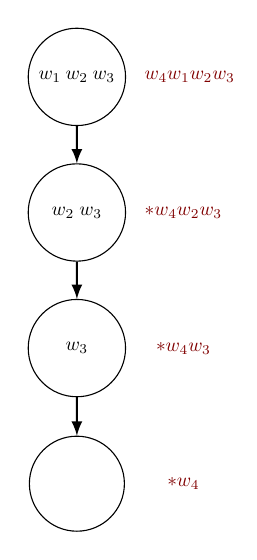
\begin{tikzpicture}
        \tikzset{
          every node/.style = {scale = 0.7},
          state/.style  = {draw, circle, align = center, text centered, text width = 4.2em},
          invis/.style  = {text width = 4.2em},
          order/.style  = {align = center, text centered, text width = 4em, text = Maroon},
        }

        \begin{scope}[node distance = 7em]
          \node [state] (highest)                    {$w_1 \: w_2 \: w_3$};
          \node [state] (lower1)  [below of=highest] {$w_2 \: w_3$};
          \node [state] (lower2)  [below of=lower1]  {$w_3$};
          \node [state] (lowest)  [below of=lower2]  {$\EmptyNGram$};
        \end{scope}

        \begin{scope}[node distance = 5.5em]
          \node [order] [right of=highest] {$\ProbMKN {w_4}{w_1 w_2 w_3}$};
          \node [order] [right of=lower1]  {$\ProbMKN*{w_4}{w_2 w_3}$};
          \node [order] [right of=lower2]  {$\ProbMKN*{w_4}{w_3}$};
          \node [order] [right of=lowest]  {$\ProbMKN*{w_4}$};
        \end{scope}

        \path[->, >=latex, thick]
          (highest) edge (lower1)
          (lower1)  edge (lower2)
          (lower2)  edge (lowest);
      \end{tikzpicture}
    \end{center}
  }
\end{frame}

\begin{frame}
  \frametitle{Generalized Language Model}

  \only<1-2>{
    \begin{align*}
      \hspace{-1.5em}
      \ProbGLM{w_n}{w_1^{n-1}} &=
        \frac{\DiscountedCount(w_1^n) + \frac{\gamma(w_1^{n-1})}{\NumSkpOp{w_1^{n-1}}}
                                        \tikzmark{recglm_high}\sum_{j=1}^{\NumSkpOp{w_1^{n-1}}} \ProbGLM*{w_n}{\SkpOp[j]{w_1^{n-1}}}}
            {\Count(w_1^{n-1} \Skp)} \\
      \intertext{\vspace{0.4cm}}
      \hspace{-1.5em}
      \ProbGLM*{w_n}{w_1^{n-1}} &=
      \frac{\DiscountedCount*(\WSkp w_1^n) + \frac{\gamma(w_1^{n-1})}{\NumSkpOp{w_1^{n-1}}}
                                              \tikzmark{recglm_low}\sum_{j=1}^{\NumSkpOp{w_1^{n-1}}} \ProbGLM*{w_n}{\SkpOp[j]{w_1^{n-1}}}}
          {\ContCountIp(\WSkp w_1^{n-1} \WSkp)}
    \end{align*}

    
\begin{tikzpicture}[
      remember picture,
      overlay,
    ]
      \draw<2>[Maroon, ultra thick] (pic cs:recglm_high) ellipse
        [xshift=6.7em, yshift=0.6ex, x radius=7.2em, y radius=4ex];
      \draw<2>[Maroon, ultra thick] (pic cs:recglm_low)  ellipse
        [xshift=6.7em, yshift=0.6ex, x radius=7.2em, y radius=4ex];
      \end{tikzpicture}
  }

  \only<3>{
    \begin{center}
      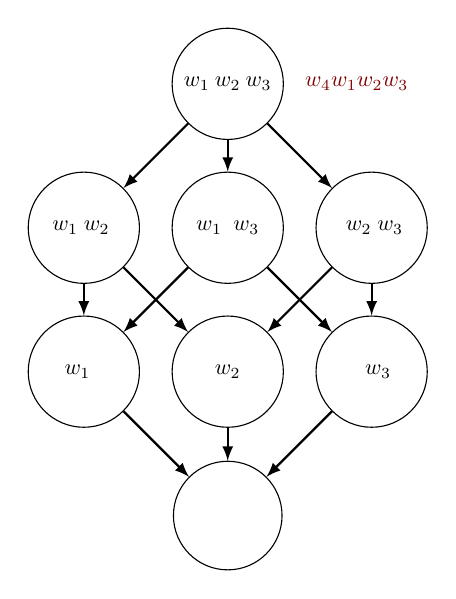
\begin{tikzpicture}
        \tikzset{
          every node/.style = {scale = 0.8},
          state/.style  = {draw, circle, align = center, text centered, text width = 4.2em},
          invis/.style  = {text width = 4.2em},
          order/.style  = {align = center, text centered, text width = 4em, text = Maroon},
        }

        \begin{scope}[node distance = 6.5em]
          \node [state] (000)                  {$w_1 \: w_2 \: w_3$};
          \node [invis] (000l) [left  of=000]  {};
          \node [invis] (000r) [right of=000]  {};

          \node [state] (001)  [below of=000l] {$w_1 \: w_2 \: \Skp$};
          \node [state] (010)  [below of=000]  {$w_1 \: \Skp \: w_3$};
          \node [state] (100)  [below of=000r] {$\Skp \: w_2 \: w_3$};

          \node [state] (011)  [below of=001] {$w_1 \: \Skp \: \Skp$};
          \node [state] (101)  [below of=010] {$\Skp \: w_2 \: \Skp$};
          \node [state] (110)  [below of=100] {$\Skp \: \Skp \: w_3$};

          \node [state] (111)  [below of=101] {$\Skp \: \Skp \: \Skp$};
          \node [invis] (111l) [below of=011] {};
          \node [invis] (111r) [below of=110] {};
        \end{scope}

        \begin{scope}[node distance = 5.5em]
          \node [order] [right of=000] {$\ProbGLM {w_4}{w_1 w_2 w_3}$};
        \end{scope}

        \path[->, >=latex, thick]
          (000) edge (001)
          (000) edge (010)
          (000) edge (100)

          (001) edge (011)
          (001) edge (101)
          (010) edge (011)
          (010) edge (110)
          (100) edge (101)
          (100) edge (110)

          (011) edge (111)
          (101) edge (111)
          (110) edge (111);
      \end{tikzpicture}
    \end{center}
  }
\end{frame}

\iffalse
\begin{frame}
  \frametitle{Backoff Graph}

  \begin{textblock}{10}(4.4,-0.9)
    \raggedleft
    \only<1>{Modified Kneser Ney Smoothing}
    \only<2>{Generalized Language Model}
  \end{textblock}

  \vspace{-0.7cm}
  \begin{center}
    \begin{tikzpicture}
      \tikzset{
        every node/.style = {scale = 0.8},
        state/.style  = {draw, circle, align = center, text centered, text width = 4.2em},
        invis/.style  = {text width = 4.2em},
        order/.style  = {align = center, text centered, text width = 4em, text = Maroon},
      }

      \only<1>{
        \begin{scope}[node distance = 7em]
          \node [state] (highest)                    {$w_1 \: w_2 \: w_3$};
          \node [state] (lower1)  [below of=highest] {$w_2 \: w_3$};
          \node [state] (lower2)  [below of=lower1]  {$w_3$};
          \node [state] (lowest)  [below of=lower2]  {$\EmptyNGram$};
        \end{scope}

        \begin{scope}[node distance = 5.5em]
          \node [order] [right of=highest] {$\ProbMKN {w_4}{w_1 w_2 w_3}$};
          \node [order] [right of=lower1]  {$\ProbMKN*{w_4}{w_2 w_3}$};
          \node [order] [right of=lower2]  {$\ProbMKN*{w_4}{w_3}$};
          \node [order] [right of=lowest]  {$\ProbMKN*{w_4}$};
        \end{scope}

        \path[->, >=latex, thick]
          (highest) edge (lower1)
          (lower1)  edge (lower2)
          (lower2)  edge (lowest);
      }

      \only<2>{
        \begin{scope}[node distance = 6.5em]
          \node [state] (000)                  {$w_1 \: w_2 \: w_3$};
          \node [invis] (000l) [left  of=000]  {};
          \node [invis] (000r) [right of=000]  {};

          \node [state] (001)  [below of=000l] {$w_1 \: w_2 \: \Skp$};
          \node [state] (010)  [below of=000]  {$w_1 \: \Skp \: w_3$};
          \node [state] (100)  [below of=000r] {$\Skp \: w_2 \: w_3$};

          \node [state] (011)  [below of=001] {$w_1 \: \Skp \: \Skp$};
          \node [state] (101)  [below of=010] {$\Skp \: w_2 \: \Skp$};
          \node [state] (110)  [below of=100] {$\Skp \: \Skp \: w_3$};

          \node [state] (111)  [below of=101] {$\Skp \: \Skp \: \Skp$};
          \node [invis] (111l) [below of=011] {};
          \node [invis] (111r) [below of=110] {};
        \end{scope}

        \path[->, >=latex, thick]
          (000) edge (001)
          (000) edge (010)
          (000) edge (100)

          (001) edge (011)
          (001) edge (101)
          (010) edge (011)
          (010) edge (110)
          (100) edge (101)
          (100) edge (110)

          (011) edge (111)
          (101) edge (111)
          (110) edge (111);
      }
    \end{tikzpicture}
  \end{center}
\end{frame}
\fi

\newcommand{\ProbMKNcab}[1]
  {\frac{\tikzmark{you_1}\DiscountedCount(\text{I love you}) + \gamma(\text{I love}) #1}{\Count(\text{I love\Skp})}}
\newcommand{\ProbMKNcb}[1]
  {\frac{\tikzmark{you_2}\DiscountedCount*(\text{\WSkp love you}) + \gamma(\text{love}) #1}{\ContCountIp(\text{\WSkp love \WSkp})}}
\newcommand{\ProbMKNc}
  {\frac{\tikzmark{you_3}\ContCountIp(\text{\WSkp you})}{\ContCountIp(\text{\WSkp \WSkp})}}

\begin{frame}
  \frametitle{Example: Probability of \enquote{you} after \enquote{I love}}

  \large
  \begin{align*}
    \hspace{-0.5cm}
    \ProbMKN {\text{you}}{\text{I love}} &= \ProbMKNcab{\ProbMKN*{\text{you}}{\text{love}}} \\
    \intertext{\vspace{0.2cm}}
    \hspace{-0.5cm}
    \ProbMKN*{\text{you}}{\text{love}}   &= \ProbMKNcb{\ProbMKN*{\text{you}}} \\
    \intertext{\vspace{0.2cm}}
    \hspace{-0.5cm}
    \ProbMKN*{\text{you}}                &= \ProbMKNc
  \end{align*}

  
\begin{tikzpicture}[
    remember picture,
    overlay,
  ]
    \draw<2->[Maroon, ultra thick] (pic cs:you_1) ellipse
      [xshift=3.2em, yshift=0.6ex, x radius=3.6em, y radius=3ex];
    \draw<2->[Maroon, ultra thick] (pic cs:you_2)  ellipse
      [xshift=3.3em, yshift=0.6ex, x radius=3.8em, y radius=3ex];
    \draw<2->[Maroon, ultra thick] (pic cs:you_3)  ellipse
      [xshift=2.6em, yshift=0.6ex, x radius=2.8em, y radius=3ex];
  \end{tikzpicture}
\end{frame}

\begin{frame}
  \frametitle{Idea: express as Weighted Sums}

  \LARGE
  \begin{equation*}
    \Prob{w}{h} = \sum_{i = 1}^{N} \tikzmark{sumweight}\SumWeight_i^h \; \tikzmark{sumarg}\SumArg_i^h(w)
  \end{equation*}

  \large
  \begin{tikzpicture}[
    remember picture,
    overlay,
    expl/.style = {draw = Maroon, rounded corners, thick},
    arrow/.style = {Maroon, thick, ->, >=latex},
  ]
    \node<2->[expl]
      (sumarg_expl) at (7.6,-1.2cm) {depends on argument $w$};
    \node<3->[expl]
      (sumweight_expl) at (6.37,3.5cm) {independent of argument $w$};
    \LARGE % restore equation size so font relative units are correct
    \draw<2->[arrow] (sumarg_expl.north)    to [out= 90, in=270] ([xshift= 1.1em, yshift=-0.9ex]{pic cs:sumarg});
    \draw<3->[arrow] (sumweight_expl.south) to [out=270, in= 90] ([xshift=-0.9em, yshift= 2.2ex]{pic cs:sumarg});
  \end{tikzpicture}
\end{frame}


% ==============================================================================
\section{Top-k Joining Techniques}
\subsection{}

\begin{frame}
  \frametitle{What are Top-k Join Queries?}

  \begin{center}
    \onslide<2->{
      \fbox{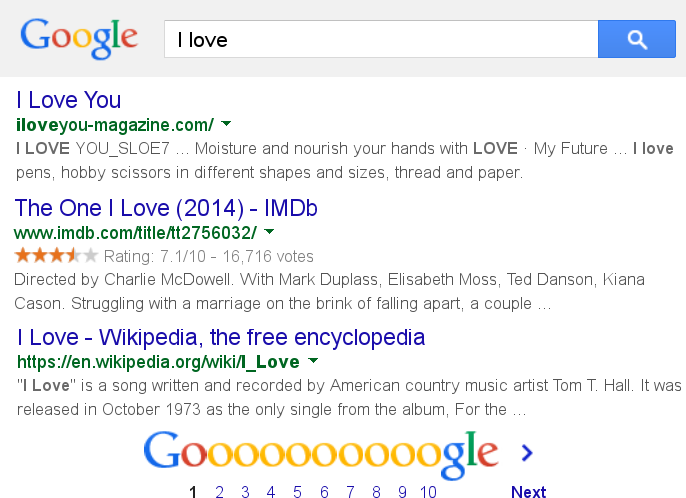
\includegraphics[width=0.8\textwidth]{figures/google-results}}}
  \end{center}

  \large
  \begin{tikzpicture}[
    remember picture,
    overlay,
    expl/.style = {draw = Maroon, rounded corners, thick, fill=white},
    arrow/.style = {Maroon, thick, ->, >=latex},
  ]
    \node<3->[expl, align=left, anchor=north] at (9cm, 7.5cm) {
      \begin{varwidth}{4.1cm}
        \vspace{0.1cm}
        \begin{itemize}
          \item like traditional\\join operations\\(e.g.\ \emph{search query})
          \only<4->{\item sorted by metric\\(e.g.\ \emph{relevance})}
          \only<5->{\item limited to $k=3$\\best results}
        \end{itemize}
        \vspace{0.1cm}
      \end{varwidth}
    };
  \end{tikzpicture}
\end{frame}

\begin{frame}
  \frametitle{Calculating probabilities for all words is slow!}

  \tabulinesep=1.5mm
  \begin{tabu}[t]{ l l }
    \action<2->{\textbf{Observation}:} &
    \action<2->{\parbox{\linewidth}{Words with high probabilities\newline
                                    have high occurrence counts\newline
                                    \small(probabilities are monotone)}} \\

    \action<3->{\textbf{Idea}:} &
    \action<3->{\parbox{\linewidth}{Keep sorted lists of occurrence counts}} \\
  \end{tabu}

  \vspace{-0.2cm}
  \onslide<3->{
    \begin{center}
      \small
      \tabulinesep=1.5mm
      \begin{tabu}{ l r | l r | l r }
        \tabucline[1pt]-
        \multicolumn{2}{ c }{$\EmptyNGram$} &
        \multicolumn{2}{ c }{love} &
        \multicolumn{2}{ c }{I love} \\
        \tabucline[1pt]-

         ~the & 50~~&
        ~~you & 30~~&
        ~~you & 25~ \\

         ~a   & 40~~&
        ~~the & 20~~&
        ~~a   &  5~ \\

         ~you & 35~~&
        ~~a   & 10~~&
        ~~the &  3~ \\
      \end{tabu}
    \end{center}}

  \vspace{-0.1cm}
  \onslide<4->{
    We apply two Top-$k$ Joining Techniques to NWP:
    \begin{itemize}
      \item Threshold Algorithm {\small\parencite{Fagin2001}}
      \item No Random Access Algorithm {\small\parencite{Fagin2001}}
    \end{itemize}}
\end{frame}



\newcommand*\Pro[1]{
  \item[\color{Pro color}\texttt{+}] \textcolor{Pro color}{#1}}
\newcommand*\Contra[1]{
  \item[\color{Contra color}\texttt{-}] \textcolor{Contra color}{#1}}
\newcommand*\Neutral[1]{
  \item[\color{black}\textbullet] \textcolor{black}{#1}}

\begin{frame}
  \frametitle{Comparison}

  \vspace{-1cm}
  \begin{columns}[t]
    \begin{column}{0.02\textwidth}\end{column}
    \begin{column}[t]{0.45\textwidth}
      \begin{center}
        \Large
        Threshold\\Algorithm
        \vspace{0.1cm} \hrule
      \end{center}

      \large
      \begin{itemize}
        \onslide<2->{\Contra{Requires Sorted and Random Access}}
        \vspace{0.3cm}
        \onslide<3->{\Pro{Faster termination}}
        \vspace{0.3cm}
        \onslide<4->{\Neutral{Needs to keep track of all seen words}}
        \vspace{0.3cm}
        \onslide<5->{\Pro{Stores at most $k$ probabilities}}
      \end{itemize}
    \end{column}
    \begin{column}{0.06\textwidth}\end{column}
    \begin{column}[t]{0.45\textwidth}
      \begin{center}
        \Large
        No Random Access\\Algorithm
        \vspace{0,1cm} \hrule
      \end{center}

      \large
      \begin{itemize}
        \onslide<2->{\Pro{Only Sorted Access necessary}}
        \vspace{0.3cm}
        \onslide<3->{\Contra{Longer runtime}}
        \vspace{0.3cm}
        \onslide<4->{\Neutral{Needs to keep track of all seen words}}
        \vspace{0.3cm}
        \onslide<5->{\Contra{Stores all seen counts plus lower and upper bounds}}
      \end{itemize}
    \end{column}
    \begin{column}{0.02\textwidth}\end{column}
  \end{columns}
\end{frame}

\begin{frame}
  \frametitle{Data structure}

  \begin{itemize}
    \item<2-> Sorted lists are unique for each history $h$
      \vspace{0.2cm}
      \begin{center}
        \small
        \tabulinesep=1.5mm
        \begin{tabu}{ l r | l r | l r }
          \tabucline[1pt]-
          \multicolumn{2}{ c }{$\EmptyNGram$} &
          \multicolumn{2}{ c }{\alert{love}} &
          \multicolumn{2}{ c }{\alert{I love}} \\
          \tabucline[1pt]-

           ~the & 50~~&
          ~~you & 30~~&
          ~~you & 25~ \\

           ~a   & 40~~&
          ~~the & 20~~&
          ~~a   &  5~ \\

           ~you & 35~~&
          ~~a   & 10~~&
          ~~the &  3~ \\
        \end{tabu}
      \end{center}
    \vspace{0.2cm}
    \item<3-> Optimized data structure: \emph{Completion Trie}\\{\small\parencite{HsuOttaviano2013}}
      \begin{itemize}
        \item Compact radix trie which stores sequence-score-pairs
        \item Optimized for prefix-retrieval
        \item Stores a minimum of edges, to achieve\\data compression and locality
        \item Variable Byte Encoding
      \end{itemize}
  \end{itemize}
\end{frame}


% ==============================================================================
\section{Evaluation}
\subsection{}

\begin{frame}
  \frametitle{Evaluation Corpus}

  \large
  Open American National Corpus {\small\parencite{OANC}}
  \begin{itemize}
    \item open collection of American English
    \item historical and contemporary
    \item spoken and written text of all genres
    \item around 600.000 sentences / 14.000.000 words
  \end{itemize}
\end{frame}

\begin{frame}
  \frametitle{Experimental Setup}

  \begin{center}
    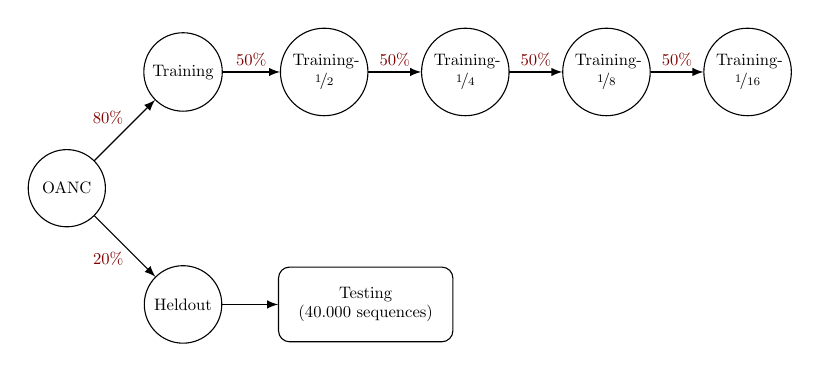
\begin{tikzpicture}
      \tikzset{
        every node/.style = {scale = 0.6},
        state/.style  = {draw, circle, align = center, text centered, text width = 3.8em},
        order/.style  = {align = center, text centered, text width = 3.8em, text = Maroon},
      }

      \begin{scope}[node distance = 7em]
        \onslide<1->{
          \node [state] (oanc)                      {OANC};
          \node         (below)    [right of=oanc]  {};
          \node [state] (training) [above of=below]  {Training};
          \node [state] (heldout)  [below of=below] {Heldout};
        }
      \end{scope}

      \begin{scope}[node distance = 8.5em]
        \onslide<2->{
          \node [state] (training2) [right of=training]  {Training-\nicefrac{1}{2}};
          \node [state] (training3) [right of=training2] {Training-\nicefrac{1}{4}};
          \node [state] (training4) [right of=training3] {Training-\nicefrac{1}{8}};
          \node [state] (training5) [right of=training4] {Training-\nicefrac{1}{16}};
        }
      \end{scope}

      \begin{scope}[node distance = 11em]
        \onslide<3->{
          \node [align=center, draw, rounded corners, minimum width = 10.5em, minimum height = 4.5em]
            (testing) [right of=heldout] {Testing\\(40.000 sequences)};
        }
      \end{scope}

      \onslide<1->{
        \path[->, >=latex]
          (oanc) edge node [above, order, xshift=-1em] {80\%} (training)
          (oanc) edge node [below, order, xshift=-1em] {20\%} (heldout);
      }

      \onslide<2->{
        \path[->, >=latex]
          (training)  edge node [above, order] {50\%} (training2)
          (training2) edge node [above, order] {50\%} (training3)
          (training3) edge node [above, order] {50\%} (training4)
          (training4) edge node [above, order] {50\%} (training5);
      }

      \onslide<3->{
        \path[->, >=latex]
          (heldout) edge (testing);
      }
    \end{tikzpicture}
  \end{center}
\end{frame}

\begin{frame}
  \frametitle{Experiments}

  TODO
\end{frame}



% ==============================================================================
\appendix
\begin{frame}[plain]
  \frametitle{So long, and thanks for all the fish}

  \begin{center}
    \textbf{Final Slide}
  \end{center}
\end{frame}


% ==============================================================================
\section{Top-k Join Examples}
\subsection{}

\begin{frame}
  \frametitle{Top-k joins combined with Weighted Sums}

  \vspace{-0.2cm}
  \onslide<2->{
    \normalsize
    \begin{equation*}
      \textstyle{\Prob{w}{h} = \sum_{i = 1}^{N} \SumWeight_i^h \; \SumArg_i^h(w)}
    \end{equation*}}

  \vspace{-0.5cm}
  \large
  \begin{itemize}
    \item<3-> Weights $\SumWeight^h_i$ can be precomputed
    \vspace{0.2cm}
    \item<4-> Sorted lists can store terms $\SumArg_i^h(w)$
  \end{itemize}

  \onslide<4->{
    \begin{center}
      \small
      \tabulinesep=1.5mm
      \begin{tabu}{ l r | l r | l r }
        \tabucline[1pt]-
        \multicolumn{2}{ c }{$\EmptyNGram$} &
        \multicolumn{2}{ c }{love} &
        \multicolumn{2}{ c }{I love} \\
        \tabucline[1pt]-

        ~the & 50~~&
        ~~\alert<6>{you} & \alert<6>{30}~~&
        ~~\alert<6>{you} & \alert<6>{25}~ \\

        ~a   & 40~~&
        ~~the & 20~~&
        ~~a   &  5~ \\

        ~\alert<6>{you} & \alert<6>{35}~~&
        ~~a   & 10~~&
        ~~the &  3~ \\
      \end{tabu}
    \end{center}}

  \large
  \begin{itemize}
    \item<5-> In examples we will assume $\SumWeight^h_1, \: \ldots, \: \SumWeight^h_N = 1$\\
      {\small(not possible in practice!)}
    \vspace{0.2cm}
    \item<6-> \alert<6>{$\Prob{\text{you}}{\text{I love}} = 35 + 30 + 25 = 95$}
  \end{itemize}
\end{frame}

\begin{frame}
  \frametitle{Threshold Algorithm}

  \begin{columns}[T]
    \begin{column}{.4\textwidth}
      \begin{enumerate}
        \item<3-> \alert< 8,12,16,18,22>{\emph{Sorted Access} to lists in any order (e.g.~round~robin)}
        \vspace{0.1cm}
        \item<4-> \alert< 9,13,19>{For new words, \emph{Random Access} to to all other lists}
        \vspace{0.1cm}
        \item<5-> \alert<11,15,17,21,23>{Compute \emph{threshold} of highest possible unseen probability}
        \vspace{0.1cm}
        \item<6-> \alert<24>{Terminate when $k$ probabilities greater threshold have been found}
      \end{enumerate}
    \end{column}
    \begin{column}{.6\textwidth}
      \onslide<1->{
        \begin{equation*}
          \textstyle{\Argmax{w \in \Vocab}\ProbMKN{w}{\text{I love}}}
        \end{equation*}}
      \vspace{-0.25cm}
      \onslide<2->{
        \tabulinesep=2mm
        \begin{tabu}{ l r | l r | l r }
          \tabucline[1pt]-
          \multicolumn{2}{ c }{$\EmptyNGram$} &
          \multicolumn{2}{ c }{love} &
          \multicolumn{2}{ c }{I love} \\
          \tabucline[1pt]-

          \tikzmark{tar1c1s} ~\action< 8->{the} & \action< 8->{50}~~\tikzmark{tar1c1e}&
          \tikzmark{tar1c2s}~~\action<12->{you} & \action<12->{30}~~\tikzmark{tar1c2e}&
          \tikzmark{tar1c3s}~~\action<13->{you} & \action<13->{25}~ \tikzmark{tar1c3e}\\

          \tikzmark{tar2c1s} ~\action<18->{a}   & \action<18->{40}~~\tikzmark{tar2c1e}&
          \tikzmark{tar2c2s}~~\action< 9->{the} & \action< 9->{20}~~\tikzmark{tar2c2e}&
          \tikzmark{tar2c3s}~~\action<19->{a}   & \action<19->{ 5}~ \tikzmark{tar2c3e}\\

          \tikzmark{tar3c1s} ~\action<13->{you} & \action<13->{35}~~\tikzmark{tar3c1e}&
          \tikzmark{tar3c2s}~~\action<19->{a}   & \action<19->{10}~~\tikzmark{tar3c2e}&
          \tikzmark{tar3c3s}~~\action< 9->{the} & \action< 9->{ 3}~ \tikzmark{tar3c3e}\\
        \end{tabu}}

        \vspace{-0.35cm}
        \begin{minipage}[t][3cm]{\textwidth}
          \begin{align*}
            \only< 7-10>{\alert< 7>{\Prob[\text{threshold}]}          &\alert< 7>{=        \infty  +        \infty  +        \infty} \hspace{-0.6em} &\alert< 7>{=}& \; \alert< 7>{\infty} \\}
            \only<11-14>{           \Prob[\text{threshold}]           &           = \alert<11>{50} +        \infty  +        \infty  \hspace{-0.6em} &           = & \;            \infty  \\}
            \only<15-16>{           \Prob[\text{threshold}]           &           =            50  + \alert<15>{30} +        \infty  \hspace{-0.6em} &           = & \;            \infty  \\}
            \only<17-20>{           \Prob[\text{threshold}]           &           =            50  +            30  + \alert<17>{25} \hspace{-0.6em} &           = & \; \alert<17>{   105} \\}
            \only<21-22>{           \Prob[\text{threshold}]           &           = \alert<21>{40} +            30  +            25  \hspace{-0.6em} &           = & \; \alert<21>{    95} \\}
            \only<14-  >{\alert<14>{\Prob{\text{you}}{\text{I love}}} &\alert<14>{=            35  +            30  +            25} \hspace{-0.6em} &\alert<14>{=}& \; \alert<14>{    90} \\}
            \only<23-  >{           \Prob[\text{threshold}]           &           =            40  + \alert<23>{20} +            25  \hspace{-0.6em} &           = & \; \alert<23>{    85} \\}
            \only<10-  >{\alert<10>{\Prob{\text{the}}{\text{I love}}} &\alert<10>{=            50  +            20  +             3} \hspace{-0.6em} &\alert<10>{=}& \; \alert<10>{    73} \\}
            \only<20-  >{\alert<20>{\Prob{\text{a  }}{\text{I love}}} &\alert<20>{=            40  +            10  +             5} \hspace{-0.6em} &\alert<20>{=}& \; \alert<20>{    55} \\}
            % For fixed alignment
            \onslide<0 >{           \Prob{\text{you}}{\text{I love}}  &           =            50  +            30  +            25  \hspace{-0.6em} &           = & \;               105}
          \end{align*}
        \end{minipage}

        
\begin{tikzpicture}[
          remember picture,
          overlay,
          iter/.style = {Maroon, thick},
        ]
          \draw< 8-17>[iter] ([yshift=-1.1ex]{pic cs:tar1c1s}) rectangle ([yshift=2.2ex]{pic cs:tar1c1e});
          \draw<12-21>[iter] ([yshift=-1.1ex]{pic cs:tar1c2s}) rectangle ([yshift=2.2ex]{pic cs:tar1c2e});
          \draw<16-  >[iter] ([yshift=-1.1ex]{pic cs:tar1c3s}) rectangle ([yshift=2.2ex]{pic cs:tar1c3e});
          \draw<18-  >[iter] ([yshift=-1.1ex]{pic cs:tar2c1s}) rectangle ([yshift=2.2ex]{pic cs:tar2c1e});
          \draw<22-  >[iter] ([yshift=-1.1ex]{pic cs:tar2c2s}) rectangle ([yshift=2.2ex]{pic cs:tar2c2e});
        \end{tikzpicture}
    \end{column}
  \end{columns}
\end{frame}


\begin{frame}
  \frametitle{No Random Access Algorithm}

  \large
  \begin{enumerate}
    \item<2-> \emph{Sorted Access} to lists in any order
    \vspace{0.3cm}
    \item<3-> Keep track of all seen counts
    \vspace{0.3cm}
    \item<4-> Compute \emph{upper} and \emph{lower bounds} for each probability
    \vspace{0.3cm}
    \item<5-> Terminate when $k$ lower bounds greater than all other upper bounds have been found
  \end{enumerate}
\end{frame}


% ==============================================================================
\section{References}
\subsection{}

\begin{frame}[allowframebreaks]
  \frametitle{References}

  \printbibliography[heading = none]
\end{frame}

\end{document}
